\documentclass[12pt, titlepage]{article}

\usepackage{booktabs}
\usepackage{tabularx}
\usepackage{hyperref}

% from SRS
\usepackage{amsmath, mathtools}
\usepackage{amsfonts}
\usepackage{amssymb}
\usepackage{graphicx}
\usepackage{colortbl}
\usepackage{xr}
\usepackage{hyperref}
\usepackage{longtable}
\usepackage{xfrac}
\usepackage{tabularx}
\usepackage{float}
\usepackage{siunitx}
\usepackage{booktabs}
\usepackage{caption}
\usepackage{pdflscape}
\usepackage{afterpage}
%%%

\usepackage{tikz}
\def\checkmark{\tikz\fill[scale=0.4](0,.35) -- (.25,0) -- (1,.7) -- (.25,.15) -- 
cycle;} 

\hypersetup{
    colorlinks,
    citecolor=black,
    filecolor=black,
    linkcolor=red,
    urlcolor=blue
}

\usepackage[round]{natbib}

\newcounter{tinnum} %Likely change number
\newcommand{\lthetinnum}{T\thetinnum}
\newcommand{\tinref}[1]{T-\ref{#1}}

%% Comments

\usepackage{color}

\newif\ifcomments\commentstrue

\ifcomments
\newcommand{\authornote}[3]{\textcolor{#1}{[#3 ---#2]}}
\newcommand{\todo}[1]{\textcolor{red}{[TODO: #1]}}
\else
\newcommand{\authornote}[3]{}
\newcommand{\todo}[1]{}
\fi

\newcommand{\wss}[1]{\authornote{blue}{SS}{#1}} 
\newcommand{\plt}[1]{\authornote{magenta}{TPLT}{#1}} %For explanation of the template
\newcommand{\an}[1]{\authornote{cyan}{Author}{#1}}

%% Common Parts

\newcommand{\progname}{Diagnose} % PUT YOUR PROGRAM NAME HERE %Every program
                                % should have a name


\begin{document}

\title{Test Report: \progname{}} 
\author{Andrea Clemeno}
\date{\today}
	
\maketitle

\pagenumbering{roman}

\section{Revision History}

\begin{tabularx}{\textwidth}{p{3cm}p{2cm}X}
\toprule {\bf Date} & {\bf Version} & {\bf Notes}\\
\midrule
December 10 & 1.0 & Initial pdf\\
December 12 & 1.1 & Notes\\
December 15 & 2.0 & Final Documentation of VnV Report\\

\bottomrule
\end{tabularx}

~\newpage

\section{Symbols, Abbreviations and Acronyms}

The table that follows summarizes the symbols used in this document along with
their descriptions. The symbols are listed in alphabetical order. In addition, 
all symbols, abbreviations, and acronyms recorded in the SRS and VnV plan for 
\progname{} 
apply to this document. Documents can be found in \citet{SRS} and 
\citet{DiagnoseVNVplan} respectively.


\begin{table}[h!]
\renewcommand{\arraystretch}{1.2}
%\noindent \begin{tabularx}{1.0\textwidth}{l l X}
\noindent \begin{longtable*}{l p{8cm}} \toprule
\textbf{symbol} & \textbf{description}\\
\midrule 
pbbt & Python Black Box Testing
\\
SRS & Software Requirements Specification
\\
T & Test 
\\
VnV & Verification and Validation 
\\
&\\
\bottomrule

\end{longtable*}
\caption{Table of Symbols, Abbreviations and Acronyms}
\end{table}

\newpage

\tableofcontents
\newpage
\listoftables %if appropriate
\newpage
\listoffigures %if appropriate
\newpage

\newpage

\pagenumbering{arabic}

This document will present the results and findings for the tests outlined in 
the VnV plan of \progname{} \citep{DiagnoseVNVplan}. The evaluation of 
functional and nonfunctional requirements with system testing methods can be 
found in 
sections \ref{fr_eval} and \ref{nfr_eval} respectively. In addition to system 
testing results, unit testing for some modules of \progname{} in section 
\ref{unittesting}. The validation of the \progname{} software
will be compared to existing data for viral load elimination from 
\citet{Stafford2000} in section \ref{validation}. Moreover, changes to the code 
with respect to these evaluations will be mentioned in section \ref{changes}. 
Lastly, the automated testing evaluations will be mentioned in section 
\ref{autotesting}.


\section{Functional Requirements Evaluation}\label{fr_eval}

\subsection{Input Verification}

These input verification tests were implemented using pbbt and verified using the methods mentioned in the VnV plan of \progname{}. Documentation of test results can be found in the 
github repository: 
\href{https://github.com/andreamclemeno/CAS741-Diagnose/tree/master/test/FunctionalReq/OutputCorrectness}{CAS741-Diagnose/test/ FunctionalReq/InputVerification}. The documentation includes input.yaml and output.yaml files that display the successful tests as well as terminal verification of passed tests.

\begin{center}
 \begin{tabular}{||c|c|c||} 
 \hline
  \bf{Test} & \bf{Test Description} & \bf{Verification Complete}\\ [0.5ex] 
  \hline
   T-1 & Expected Input & \checkmark \\
  \hline
   T-2 & Invalid Input: $N_{o}$ & \checkmark \\
  \hline
   T-3 & Invalid Input: $N_{t}$ & \checkmark \\
  \hline
   T-4 & Invalid Inputs: $N_{o}$, $N_{t}$ & \checkmark \\
  \hline
   T-5 & Invalid Input: $t_{t}$ & \checkmark \\
  \hline
   T-6 & Invalid Input: $t_{d}$ & \checkmark \\
  \hline
   T-7 & Invalid Inputs: $t_{t}$, $t_{p}$ & \checkmark \\
  \hline
\end{tabular}
\captionof{table}{Functional Requirements Evaluation: Input Verification}
\label{table_inputverification}

\end{center}	

\subsection{Output Correctness}

This output correctness test was implemented using pbbt and verified using the methods mentioned in the VnV plan of \progname{}. Documentation of test results can be found in the 
github repository: 
\href{https://github.com/andreamclemeno/CAS741-Diagnose/tree/master/test}{CAS741-Diagnose/test/ FunctionalReq/OutputCorrectness}. The documentation includes input.yaml and output.yaml files that display the successful tests as well as terminal verification of passed tests.

\begin{center}
 \begin{tabular}{||c|c|c||} 
 \hline
  \bf{Test} & \bf{Test Description} & \bf{Verification Complete}\\ [0.5ex] 
  \hline
   T-8 & Expected Input & \checkmark \\
  \hline
\end{tabular}
\captionof{table}{Functional Requirements Evaluation: Output Correctness}
\label{table_outputcorrectness}

\end{center}	


\section{Nonfunctional Requirements Evaluation}\label{nfr_eval}
		
\subsection{Understandability}

A successful test is specified by the automatic verification of no error 
messages in the linting process. The static analysis run in the Spyder IDE found 
no error messages seen in table \ref{lintingresults}. Overall, the verification 
of understandability has been successful as seen in table 
\ref{table_understandability}. Documentation of test results can be found on the 
github repository: 
\href{https://github.com/andreamclemeno/CAS741-Diagnose/tree/master/test/NonfunctionalReq/NFR1-Understandability}{CAS741-Diagnose/test/NonfunctionalReq/NFR1-Understandability/}. Documentation includes .pylintrc files that display the output of linting.

\begin{center}
 \begin{tabular}{||c|c|c|c|c|c||} 

 \hline
  \bf{Module} & \bf{Conventions} & \bf{Refactoring} & \bf{Warnings} & 
\bf{Errors} & \bf{Global Eval.}\\ [0.5ex] 
  \hline
   Control.py & 8  & 0 & 0 & 0 & 7.14\\
  \hline
   Calculations.py & 9  & 0 & 0 & 0 & 5.50\\
  \hline
   InputFormat.py & 5 & 0 & 0 & 0 & 8.75\\
  \hline
   InputParameters.py & 3  & 1 & 1 & 0 & -15.00\\
  \hline
   InputConstraints.py & 17 & 0 & 0 & 0 & 5.50\\
  \hline
   OutputFormat.py & 5 & 0 & 0 & 0 & 6.88\\
  \hline
\end{tabular}
\captionof{table}{Linting Results}\label{lintingresults}
\end{center}	

\begin{center}
 \begin{tabular}{||c|c|c||} 
 \hline
  \bf{Test} & \bf{Test Description} & \bf{Verification Complete}\\ [0.5ex] 
  \hline
   T-9 & Linting for \progname{} Modules   & \checkmark \\
  \hline
\end{tabular}
\captionof{table}{Non-functional Requirements Evaluation: Understandability}
\label{table_understandability}
\end{center}	


\subsection{Reliability}

A successful test is specified by the verification of a total run time 
of less than 0.1 seconds. As seen in Figure \ref{Fig_cprofile}, the run time is 
0.007 seconds and passes the reliability test. Overall, the verification of 
reliability has been successful as seen in table \ref{table_reliability}. 
Documentation of test results can be found on the github repository: 
\href{https://github.com/andreamclemeno/CAS741-Diagnose/tree/master/test/NonfunctionalReq/NFR2-Reliability}{CAS741-Diagnose/test/NonfunctionalReq/NFR2-Reliability}. The documentation includes a text file with the terminal output of the cProfile command.

 \begin{figure}[H]
 \begin{center}
 %\rotatebox{-90}
 {
  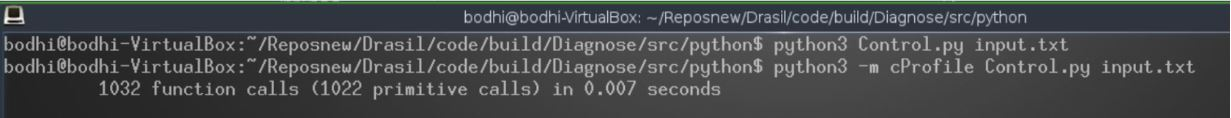
\includegraphics[width=1\textwidth]{cprofile.JPG}
 }
 \caption{Reliability Test: Dynamic Analysis using cProfile}

 \label{Fig_cprofile}
 \end{center}
 \end{figure}


\begin{center}
 \begin{tabular}{||c|c|c||} 
 \hline
  \bf{Test} & \bf{Test Description} & \bf{Verification Complete}\\ [0.5ex] 
  \hline
   T-10 & Reliability   & \checkmark \\
  \hline
\end{tabular}
\captionof{table}{Non-functional Requirements Evaluation: Reliability}
\label{table_reliability}
\end{center}	


\subsection{Maintainability}

Testing for maintainability involves the manual verification of traceability 
from tests to requirements seen in table \ref{Table:R_trace} and traceability 
from tests to modules seen in table \ref{Table:M_trace}. From these tables,
it is seen that each requirement and module is tested. In addition, traceability 
matrices in the SRS and VnV document are completed and demonstrate traceability 
to 
ensure maintainability of the software \citep{DrasilSRS}. Overall, the 
verification of 
maintainability has been successful as seen in table 
\ref{table_maintainability}.

\begin{center}
 \begin{tabular}{||c|c|c||} 
 \hline
  \bf{Test} & \bf{Test Description} & \bf{Verification Complete}\\ [0.5ex] 
  \hline
   T-11 & Maintainability   & \checkmark \\
  \hline
\end{tabular}
\captionof{table}{Non-functional Requirements Evaluation: Maintainability}
\label{table_maintainability}
\end{center}	

\subsection{Portability}

A successful test is specified by the completion of the make command. 
As seen in table \ref{table_os}, the make is completed for Windows OS and 
Linux OS, and passes the portability test. Overall, the verification of 
portability has been successful as seen in table \ref{table_portability}.

\begin{center}
 \begin{tabular}{||c|c||} 
 \hline
  \bf{OS}  & \bf{Make Completed}\\ [0.5ex] 
  \hline
    Windows OS  & \checkmark \\
  \hline
    Linux OS    & \checkmark \\
  \hline
\end{tabular}
\captionof{table}{Portability test: OS and Make Completion}
\label{table_os}
\end{center}	


\begin{center}
 \begin{tabular}{||c|c|c||} 
 \hline
  \bf{Test} & \bf{Test Description} & \bf{Verification Complete}\\ [0.5ex] 
  \hline
   T-12 & Portability   & \checkmark \\
  \hline
\end{tabular}
\captionof{table}{Non-functional Requirements Evaluation: Portability}
\label{table_portability}
\end{center}	

\subsection{Verifiability}

Successful verification testing is indicated by the successful manual 
verification of tests T-1 to T-15. The verifiability of functional requirements 
is determined by the verification of functional requirement system testing seen 
in section \ref{fr_eval} and unit testing seen in section \ref{unittesting}. The 
verifiability of nonfunctional requirements is determined by the verification of 
non-functional requirement system testing seen in section \ref{nfr_eval}. 
Overall, the verification of verifiability has been successful as seen in table 
\ref{table_verifiability}.

\begin{center}
 \begin{tabular}{||c|c|c||} 
 \hline
  \bf{Test} & \bf{Test Description} & \bf{Verification Complete}\\ [0.5ex] 
  \hline
   T-13 & Verifiability of Functional Requirements  & \checkmark \\
  \hline
   T-14 & Verifiability of Nonfunctional Requirements   & \checkmark \\
  \hline
\end{tabular}
\captionof{table}{Non-functional Requirements Evaluation: Verifiability}
\label{table_verifiability}
\end{center}	

\section{Comparison to Existing Implementation}\label{validation}

The validation of \progname{} was completed by comparing the outputs of the 
software to several cases from scientific study called Modeling plasma virus 
concentration during primary HIV infection seen in The Journal of Theoretical 
Biology
\citep{Stafford2000}. For more documentation of validation results can be found on the github repository: 
\href{https://github.com/andreamclemeno/CAS741-Diagnose/tree/master/test}{andreamclemeno/CAS741-Diagnose/test}.

The validation was completed using patient 1-4 and 6-10 data from \citet{Stafford2000} seen in table \ref{patient}. For simplicity, patient 1-4 and 6-10 will be referred to as patients 1-7.

\begin{center}
 \begin{tabular}{||c||c|c|c|c||} 
 \hline
  \bf{Patient}  & \textbf{$N_{o}$ ($\frac{mol}{mL}$)} & \textbf{$N_{t}$ ($\frac{mol}{mL}$)} & \textbf{$t_{t}$ (d)} & \textbf{$t_{p}$ (d)}\\ [0.5ex] 
  \hline
   1 & 94760000	 & 70620000	 & 2 & 8\\
  \hline
   2 & 28400000	 & 21600000	 & 1 & 9\\
  \hline
   3 & 148500000	 & 70160000	 & 5 & 7\\
  \hline
   4 & 239860000	 & 33720000	 & 5 & 8\\
  \hline
   5 & 242790000	 & 220040000	 & 3 & 7\\
  \hline
   6 & 35540000	 & 14680000 & 4 & 11\\
  \hline
   7 & 962280000 & 783000000	 & 1 & 5\\
  \hline
\end{tabular}
\captionof{table}{Software Validation: Patient 1-9 data}
\label{patient}
\end{center}	

The data from table \ref{patient} is compared with data from the \progname{} software and the theoretical error is found and presented in table \ref{comparestudy}. Additionally, \href{https://github.com/andreamclemeno/CAS741-Diagnose/tree/master/test}{andreamclemeno/CAS741-Diagnose/test} contains graphs for easier comparison. An example of patient 7 can be seen in figure \ref{Fig_graphexample}.  

\begin{center}
 \begin{tabular}{||c||c|c|c||} 
 \hline
  \bf{Patient}  & \textbf{Strafford $N_{p}$ ($\frac{mol}{mL}$)} & \textbf{Diagnose $N_{p}$ ($\frac{mol}{mL}$)} & \textbf{$error$ (d)} \\ [0.5ex] 
  \hline
   1 & 144000	 & 2.2094e-16	 & 6.5174e+23 \\
  \hline
   2 & 	143000 & 1.4870e-07	 &  9.6165e+15\\
  \hline
   3 & 	564000 & 7.9327e-13	 &  7.1097+21\\
  \hline
   4 & 	340600 & 0.3354	 &  1.0152e+10\\
  \hline
   5 & 1134300	 & 4.8829e-85	 &  2.3229e+94\\
  \hline
   6 & 100900	 & 8.6790e-15 &  1.1625e+23\\
  \hline
   7 & 7158100 & 0.0282	 &  2.5339e+11\\
  \hline
\end{tabular}
\captionof{table}{Software Validation: Viral Load from \citet{Stafford2000} vs  Diagnose}
\label{comparestudy}
\end{center}	

\begin{figure}[h!]
 \begin{center}
 %\rotatebox{-90}
 {
  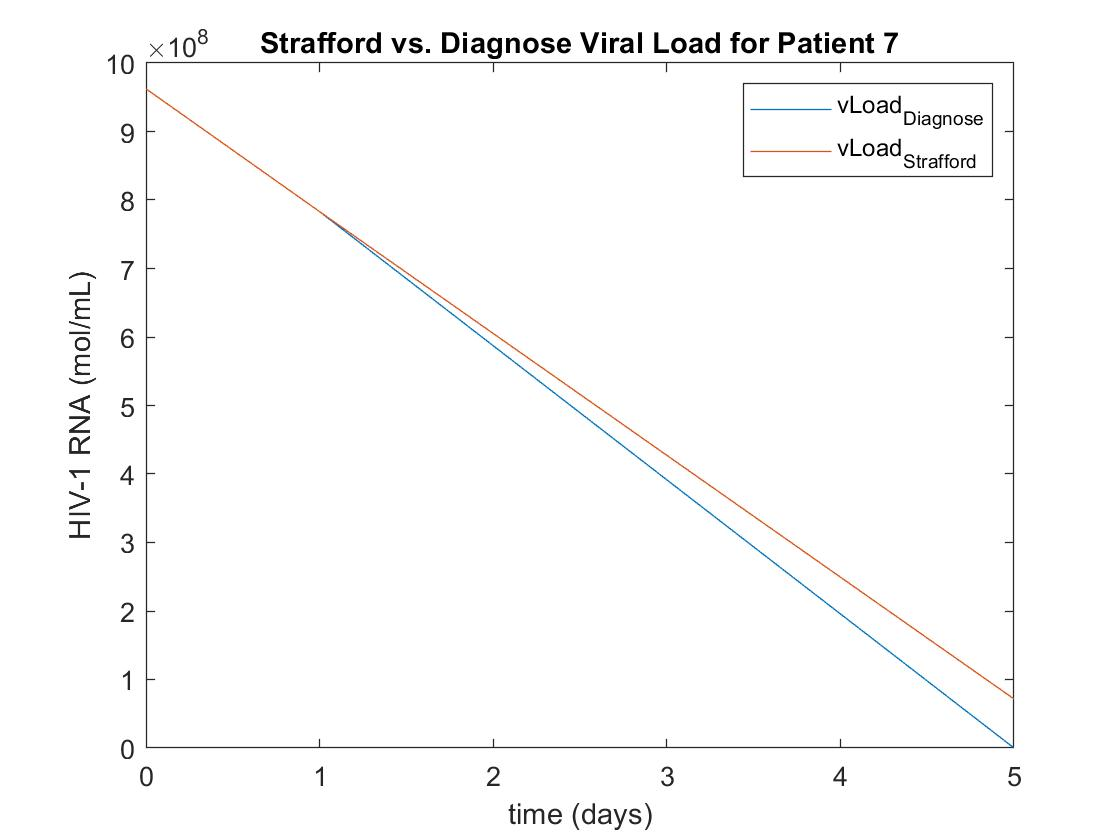
\includegraphics[width=1\textwidth]{graphexample.jpg}
 }
 \caption{Viral Load from \citet{Stafford2000} vs  Diagnose: Patient 7}

 \label{Fig_graphexample}
 \end{center}
 \end{figure}



\section{Unit Testing}\label{unittesting}

\subsection{Calculations Module}

Unit testing for Calculations.py was completed using unittest in the Spyder IDE. 
Exceptions were raised if the module was not behaving properly. For T-14, the 
test cases displayed the OK indicator classifying the test as successful as seen 
for testcase7b.txt in Figure \ref{Fig_unittestexample}. Overall, the unit test 
cases were successful as seen in table \ref{table_unit}. Documentation of test 
results can be found on the github repository: \href{https://github.com/andreamclemeno/CAS741-Diagnose/tree/master/test/UnitTesting}{CAS741-Diagnose/test/UnitTesting}. The documentation includes the output of all test cases mentioned in the VnV plan \citep{DiagnoseVNVplan}.

 \begin{figure}[h!]
 \begin{center}
 %\rotatebox{-90}
 {
  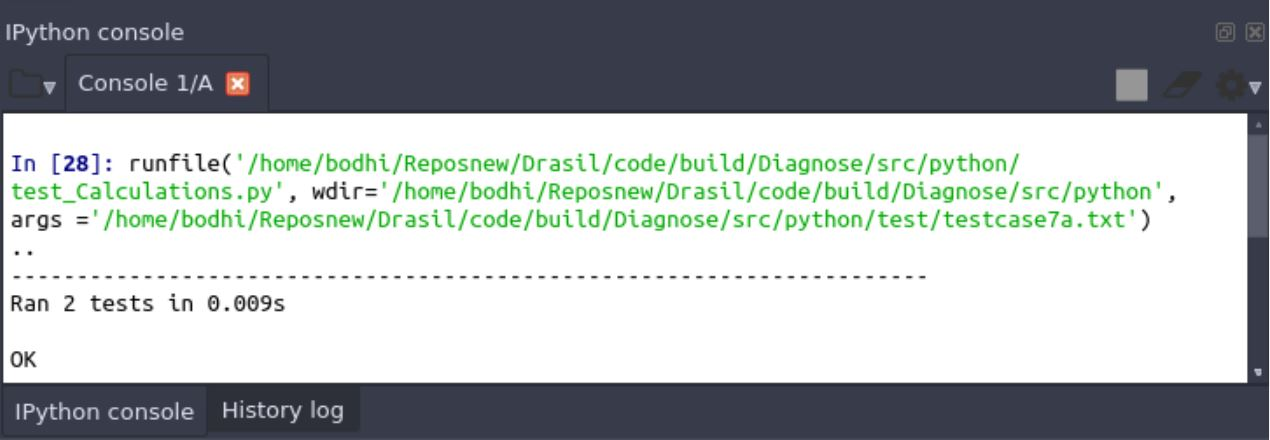
\includegraphics[width=1\textwidth]{unittestexample.jpg}
 }
 \caption{Unit Test Example: Calculations.py, testcase7b.txt}

 \label{Fig_unittestexample}
 \end{center}
 \end{figure}


\begin{center}
 \begin{tabular}{||c|c|c||} 
 \hline
  \bf{Test} & \bf{Test Description} & \bf{Verification Complete}\\ [0.5ex] 
  \hline
   T-15 & Test for Calculations.py & \checkmark \\
  \hline
\end{tabular}
\captionof{table}{Unit testing Evaluation}
\label{table_unit}

\end{center}	

\section{Changes Due to Testing}\label{changes}

No major changes were implemented due to testing. However, during the linting 
process, the variable of elimination rate was changed from $\lambda$ to $k$ as 
ASCII characters are did not follow coding standards.

\section{Automated Testing}\label{autotesting}

The automated testing tool used by \progname{} is Travis CI. The build can be 
found on the github repository: \href{https://github.com/andreamclemeno/Drasil}{andreamclemeno/Drasil}. The build has not completed as of December 15, 2020 due to redundant brackets and error in adding author information. 

		
\section{Trace to Requirements}


The purpose of the traceability matrices is to provide easy references on what
has to be additionally modified if a certain component is changed.  Every time a
component is changed, the items in the column of that component that are marked
with an ``X'' may have to be modified as well.  Table~\ref{Table:R_trace} shows 
which test cases are supporting which requirements.



\begin{table}[H]
\centering
\begin{tabular}{||c||c|c|c|c|c|c|c|c|c|c||}
\hline
	& R1 & R2 & R3 & R4 & R5 & NF1 & NFR2 & NFR3 & NFR4 & NFR5 \\
\hline
T-1        	& X& X& X& X& X& & & & & \\
\hline
T-2			& X& X& & & & & & & &\\
\hline
T-3        	& X& X& & & & & & & &\\
\hline
T-4			& X& X& & & & & & &  &\\
\hline
T-5       	& X& X& & & & & & & &\\
\hline
T-6			& X& X& & & & & & & &\\
\hline
T-7        	& X& X& & & & & & & &\\
\hline
T-8			& X& X&X & X& X& & & & &\\ 
\hline
T-9        	& & & & & &X & & & &\\
\hline
T-10 		& & & & & &X & & & &\\
\hline
T-11        	& & & & & & &X & & &\\
\hline
T-12			& & & & & & & &X & &\\ 
\hline
T-13        	& & & & & & & & &X &\\
\hline
T-14			& & & & & & & & & &X\\
\hline
T-15        	& & &X & & & & & & &\\
\hline

\end{tabular}
\caption{Traceability Matrix Showing the Connections Between Requirements and 
Tests}
\label{Table:R_trace}
\end{table}
		
\section{Trace to Modules}	


The purpose of the traceability matrices is to provide easy references on what
has to be additionally modified if a certain component is changed.  Every time a
component is changed, the items in the column of that component that are marked
with an ``X'' may have to be modified as well.  Table~\ref{Table:M_trace} shows 
which test are supporting which modules.

\begin{landscape}
\begin{table}[ht]
\centering
\begin{tabular}{||c||c|c|c|c|c|c||}
\hline
	& Calculations.py & Control.py & InputConstraints.py & InputFormat.py & 
InputParameter.py & OutputFormat.py \\
\hline
T-1        	&X &X &X &X &X &X  \\
\hline
T-2			& & & & & &  \\
\hline
T-3        	& & & & & &  \\
\hline
T-4			& & & & & &  \\
\hline
T-5        	& & & & & &  \\
\hline
T-6			& & & & & &  \\
\hline
T-7			& & & & & &  \\
\hline
T-8			&X &X &X &X &X &X  \\
\hline
T-9			& & & & & &  \\
\hline
T-10			& & & & & &  \\
\hline
T-11			& & & & & &  \\
\hline
T-12			& & & & & &  \\
\hline
T-13			& & & & & &  \\
\hline
T-14			& & & & & &  \\
\hline
T-15			& & &X & & &  \\
\hline
\end{tabular}
\caption{Traceability Matrix Showing the Connections Between Modules and 
Tests}
\label{Table:M_trace}
\end{table}
\end{landscape}	

\bibliographystyle{plainnat}

\bibliography{references.bib}
~\newpage

\end{document}



